\chapter{Planificación}

\section{Fases}

Las fases seguidas a lo largo del desarrollo de este proyecto son las que se detallan a continuación:

\begin{itemize}
	\item \textbf{Fase 1:} Espeficiación del proyecto. Se establecen los objetivos a cumplir para que el proyecto se considere completado con éxito, entendiendo que se satisfacen todos los requisitos y funcionalidades.
	\item \textbf{Fase 2:} Planificación. Se definen las fases de desarrollo del sistema y las actividades a desarrollar en cada una de ellas.
	\item \textbf{Fase 3:} Análisis. Se realiza el análisis de requisitos del sistema. 
	\item \textbf{Fase 4:} Adquisición del conocimiento. Se obtienen los conocimientos necesarios para poder crear el sistema experto.
	\item \textbf{Fase 5:} Diseño. Se analizan todos los aspectos del proyecto para concretar su desarrollo.
	\item \textbf{Fase 6:} Implementación. Se procede a implementar todas las funcionalidades necesarias.
	\item \textbf{Fase 7:} Pruebas y validación. Se verifica y valida el sistema para comprobar su correcto funcionamiento.
	\item \textbf{Fase 8:} Documentación. Se realiza toda la documentación informativa y explicativa.
\end{itemize}

Aunque parece que estas fases se llevan a cabo de forma lineal, esto no es completamente cierto. La fase de aquisición del conocimiento se lleva a cabo a lo largo de todo el proceso de desarrollo de sistema. Esto se debe al hecho de que al necesitar conocimientos expertos específicos y externos, no conocidos por el desarrollador, es necesario realizar este proceso de adquisición paralelamente al resto de tareas para poder construir de forma correcta el sistema, de acuerdo al ámbito de conocimiento del mismo.

Esto hace que el proceso sea más complejo al tener que hacer una revisión, adquisición y comprensión continúa de conocimientos ajenos a la ingeniería informática. 

\section{Lista de tareas}

\begin{itemize}
	\item \textbf{Especificación del proyecto:}
	\begin{itemize}
		\item Determinación de objetivos. Se definen los objetivos que se quieren alcanzar con el desarrollo de este proyecto.
		\item Determinación de requisitos. Se definen los requisitos que se deben satisfacer para alcanzar los objetivos definidos.
	\end{itemize}
\end{itemize}

\bigskip

\begin{itemize}
	\item \textbf{Planificación:}
	\begin{itemize}
		\item Lista de actividades. Se especifican las actividades y tareas que deben llevarse a cabo en cada fase del desarrollo.
		\item Recursos humanos. Se especifica el personal que va a participar en el desarrollo del proyecto y sus funciones.
		\item Temporización. Se determinan los plazos y fechas para la ejecución de cada una de las fases del proyecto.
	\end{itemize}
\end{itemize}

\bigskip

\begin{itemize}
	\item \textbf{Análisis:}
	\begin{itemize}
		\item Análisis de requisitos. Se definen los requisitos de información, funcionales y no funcionales del sistema.
		\item Descripción de casos de uso. Se describen los casos de uso del sistema.
		\item Diagramas de casos de uso. 
		\item Diagramas de actividad.
	\end{itemize}
\end{itemize}

\bigskip

\begin{itemize}
	\item \textbf{Adquisición del conocimiento:}
	\begin{itemize}
		\item Extracción de conocimientos. Se especifica el proceso de adquisición de conocimientos de diversas fuentes no humanas.
		\item Educción de conocimientos. Se especifica el proceso de adquisición de conocimientos de diversos expertos.
		\item Estructuración de conocimientos. Se especifican los hechos y reglas que componen el sistema.
	\end{itemize}
\end{itemize}

\bigskip

\begin{itemize}
	\item \textbf{Diseño:}
	\begin{itemize}
		\item Selección de herramientas. Se describe el proceso de elección de herramientas para el desarrollo, tanto del sistema experto como de su interfaz.
		\item Diseño de la arquitectura. Se definen los componentes y módulos estructurales del sistema y las relaciones entre los mismos.
	\end{itemize}
\end{itemize}

\bigskip

\begin{itemize}
	\item \textbf{Implementación:}
	\begin{itemize}
		\item Implementación del sistema experto. Se describe el proceso de implementación del sistema, así como todos los problemas surgidos durante el mismo y las soluciones aplicadas.
		\item Implementación de la interfaz. Se describe el proceso de implementación de la interfaz, así como todos los problemas surgidos durante el mismo y las soluciones aplicadas.
	\end{itemize}
\end{itemize}

\bigskip

\begin{itemize}
	\item \textbf{Pruebas y validación:}
	\begin{itemize}
		\item Verificación. Se comprueba el funcionamiento y comportamiento del sistema.
		\item Validación del sistema por un experto. Se comprueba que el funcionamiento del sistema es correcto.
	\end{itemize}
\end{itemize}

\bigskip

\begin{itemize}
	\item \textbf{Documentación:}
	\begin{itemize}
		\item Documentación del proyecto. Se procede a registrar y explicar todo el proceso de desarollo así como las decisiones tomadas a lo largo del mismo.
	\end{itemize}
\end{itemize}

\section{Recursos humanos}

Para poder desarrollar este proyecto he contado con la ayuda de varios músicos y compositores profesionales que me han ayudado a crear la base de conocimiento del sistema. Además, también he contado con profesores del Conservatorio Profesional de Música Ángel Barrios de Granada para poder llevar a cabo su validación.

Los expertos consultados han sido:

\begin{itemize}
	\item Alberto José Moreno Montes (Violista y compositor)
	\item Isabel Salado Ortega (Pianista)
	\item Clara Luz Fernández Vecino (Profesora de armonía)
\end{itemize}

El tener varios expertos a los que consultar y especializados en diferentes áreas musicales hace que podamos construir una base de conocimiento mucho más amplia, consistente y mejor estructurada. Sin embargo, esto también supone una dificultad añadida. Ésta radica en el hecho de que, como se menciona en la introducción, algunos aspectos referidos a la música poseen un carácter subjetivo y cada experto puede tener opiniones o percepciones distintas sobre algunos conceptos o situaciones específicas. Teniendo en cuenta esto, tener una mayor cantidad de información y conocimientos que aprehender y seleccionar de cara a nuestro sistema puede suponer un proceso largo y complejo, incluso una ``desventaja'', pero hace que el sistema sea mucho más completo y preciso a la hora de deducir y obtener conclusiones.

\section{Temporización}

Para percibir de forma más visual la planificación estructural y temporal en las figuras \ref{fig1.4.1}, \ref{fig1.4.2} y \ref{fig1.4.3} se muestran una serie de diagramas.

\begin{figure}[H]
	\centering
	\hspace*{-1.2in}
	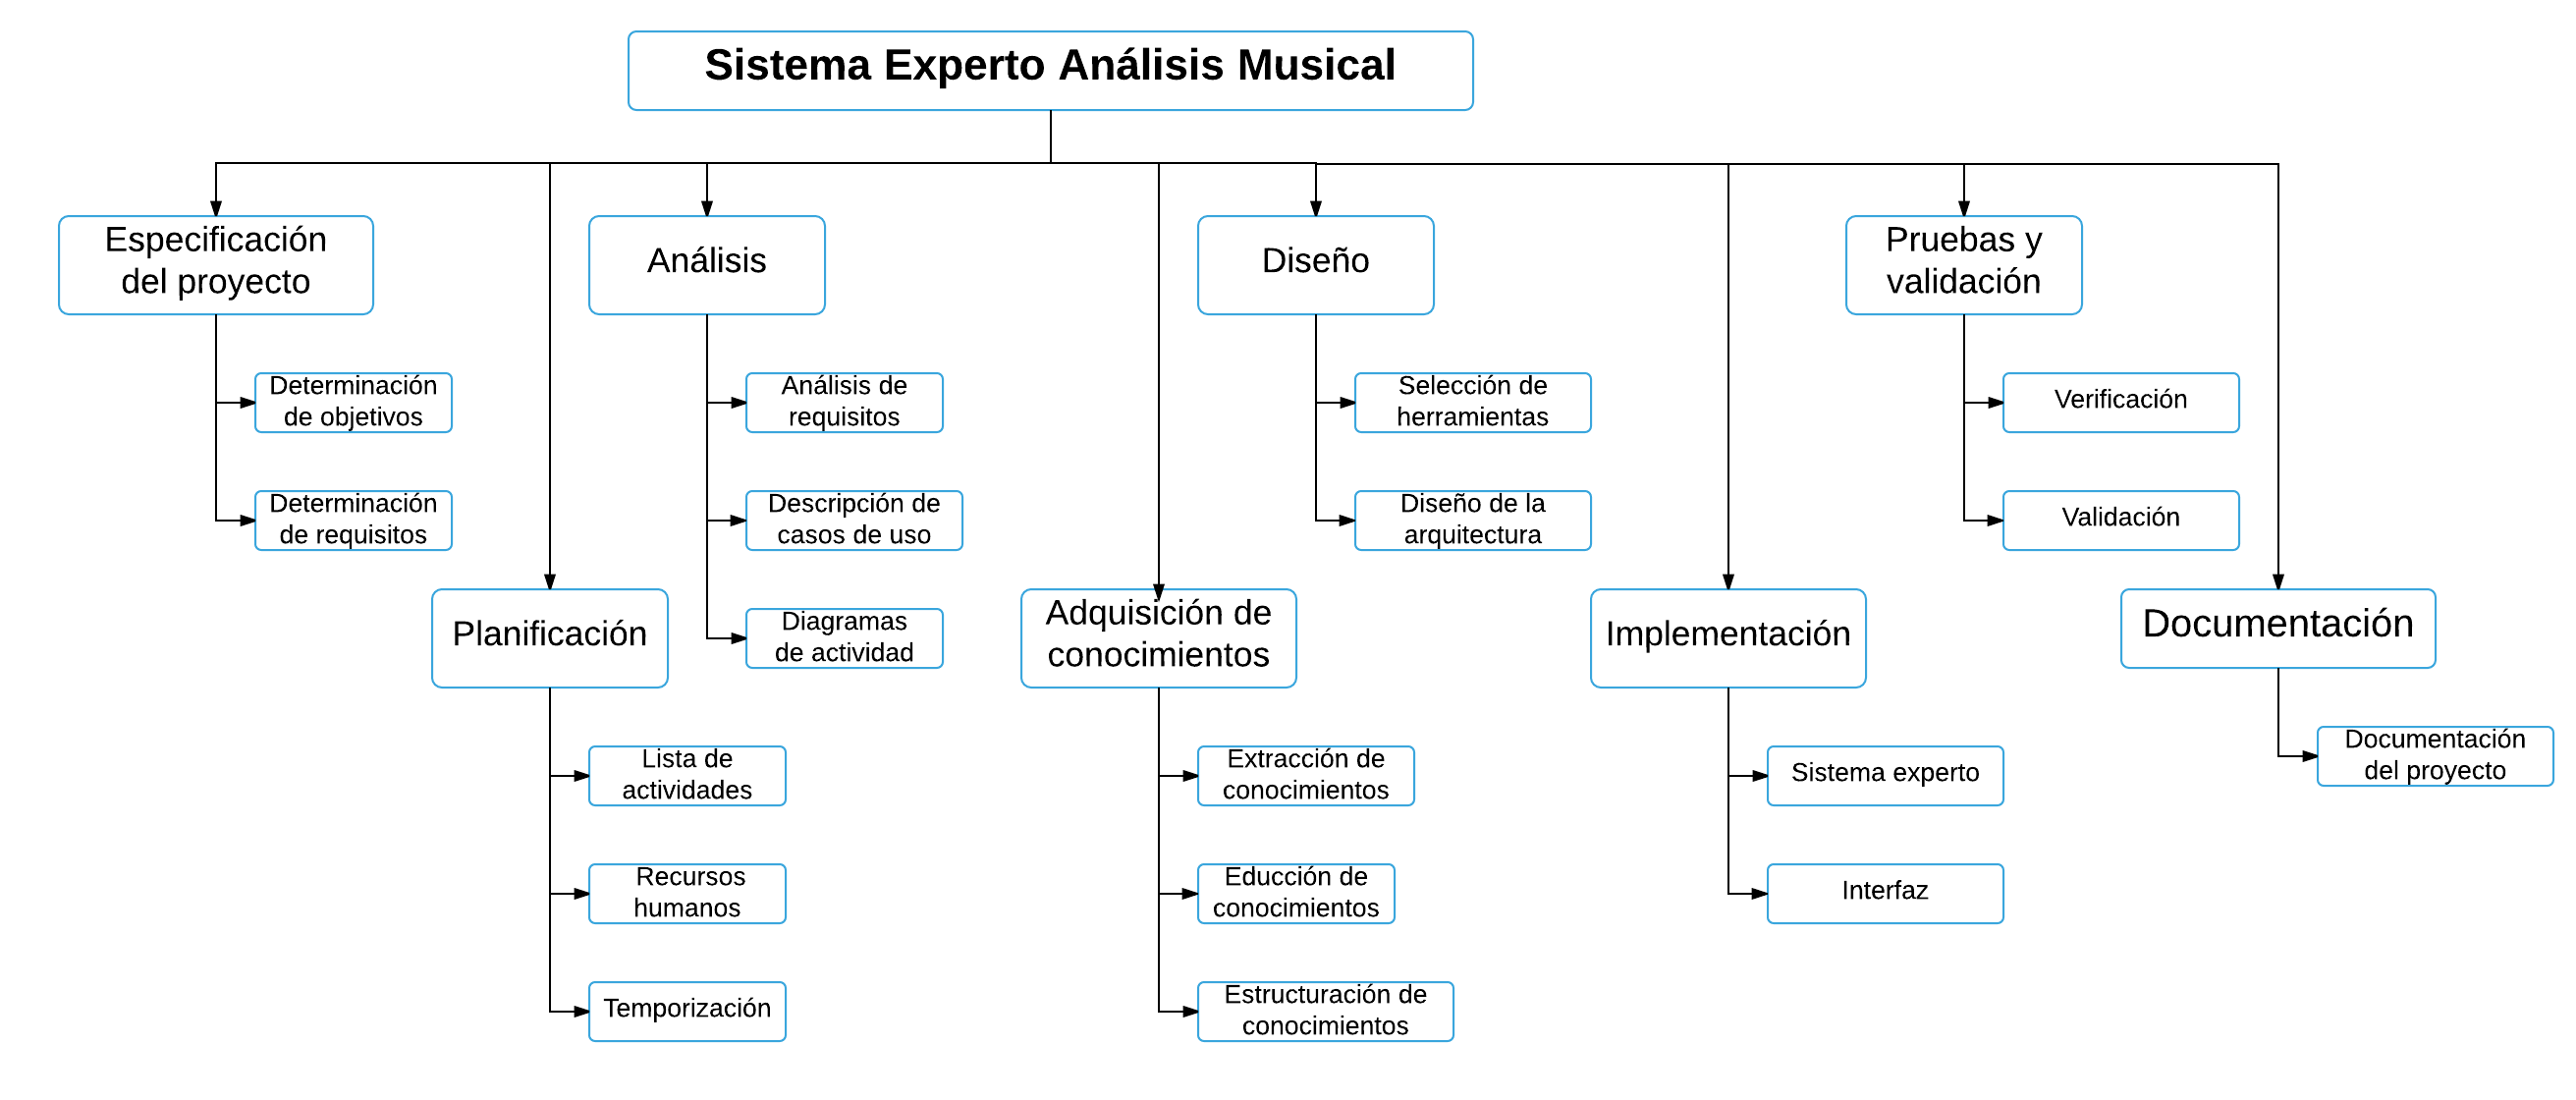
\includegraphics[scale=0.5]{imagenes/diagrama_edt.png}
	\caption{Diagrama de estructura de descomposición de trabajo}
	\label{fig1.4.1}
\end{figure}

\begin{figure}[H]
	\centering
	\hspace*{-0.6in}
	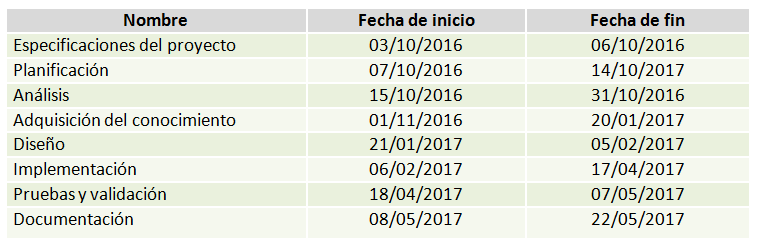
\includegraphics[scale=0.7]{imagenes/diagrama_tareas.png}
	\caption{Temporización de las tareas}
	\label{fig1.4.2}
\end{figure}

\bigskip
\bigskip

\begin{figure}[H]
	\centering
	\hspace*{-0.6in}
	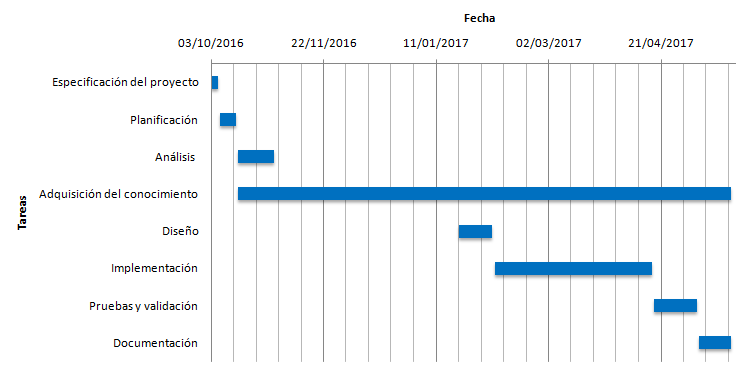
\includegraphics[scale=0.80]{imagenes/diagrama_gantt.png}
	\caption{Diagrama de Gantt}
	\label{fig1.4.3}
\end{figure}